\section{Experiments}

\newcommand{\mc}[1]{{\color{red} --- MC: #1 ---}}

\graphicspath{{../imgs/}}

\newcommand{\data}[1]{\texttt{#1}}
\newcommand{\higgs}{\texttt{Higgs}\xspace}
\newcommand{\phones}{\texttt{Phones}\xspace}
\newcommand{\wiki}{\texttt{Wiki}\xspace}
\newcommand{\chen}{\textsc{ChenEtAl}\xspace}
\newcommand{\seq}{\textsc{SeqCoreset}\xspace}
\newcommand{\stream}{\textsc{StremingCoreset}\xspace}
\newcommand{\mapr}{\textsc{MRCoreset}\xspace}

With this experimental evaluation, we aim to answer the following questions:
\begin{itemize}
    \item What is the influence of the coreset size on the performance, 
        both in terms of quality and running time?
    \item How does the coreset-based strategy compare with the algorithm 
        by Chen et al.~\cite{DBLP:journals/algorithmica/ChenLLW16}?
    \item How do \stream and \seq compare in terms of memory requirements?
    \item How expensive is to build the coreset, compared with finding
        a good clustering on the coreset itself?
    \item How does the coreset construction benefit from parallelism?
\end{itemize}

\paragraph*{Experimental setup}
We implemented all algorithms using Rust 1.53.0-nightly (\texttt{ca075d268} 2021-04-28).
The MapReduce implementation runs on top of Timely Dataflow~\cite{DBLP:journals/cacm/MurrayMIIBA16}.
All experiments have been executed on a cluster with 8 machines equipped
with a Intel\textregistered Xeon\textregistered CPU (E5-2670 v2 @ 2.50GHz), and 16 Gb of RAM each.

Our open source implementation is available at~\url{https://github.com/Cecca/macaco}.
As an optimization for the \stream algorithm, instead of updating the independent set associated to a cluster center on every node addition
-- which involve calling the expensive matroid oracle -- we buffer the points for each cluster center,
computing the independent set only once every 2048 additions.

In all experiments, rather than setting the parameter $\epsilon$, which in the previous sections 
relates the quality of the solution with the size of the coreset, we control directly the number of 
cluster centers around which the coresets are built. We denote this parameter with $\tau$.
This is to have greater control on the size of the coreset, with the goal of observing the
effect on the performance both in terms of time and quality.
Each result is the average over at least 10 runs.

\begin{table}
    \caption{\label{tab:datasets}Datasets used in this experimental evaluation.}
    \begin{tabular}{lrrlr}
        \toprule
        dataset & n & dim & matroid & rank \\
        \midrule
        \higgs & 11\,000\,000 & 7 & Partition & 20  \\ 
        \phones & 13\,062\,475 & 3 & Partition & 35 \\ 
        \wiki & 4\,976\,753 & 10 & Transversal & 50 \\ 
        \bottomrule
    \end{tabular}
\end{table}
\paragraph*{Datasets}
We consider three datasets in this experimental evaluation, whose characteristics are summarised
in Table~\ref{tab:datasets}.
The scripts to download and preprocess the datasets are available in the code repository.

\higgs\footnote{\url{https://archive.ics.uci.edu/ml/datasets/HIGGS}}
is a dataset of simulated readings from a particle detector. Each set of readings is classified as
being either \emph{signal} or \emph{background}. We define a partition matroid on these two classes
by allowing 10 points from each.

\phones\footnote{\url{https://archive.ics.uci.edu/ml/datasets/Heterogeneity+Activity+Recognition}} 
is a dataset of sensor readings from phones, each tagged with one of seven activities 
(stand, sit, walk, bike, stairs up, stairs down, \emph{null}). We define a partition matroid on
these activities by allowing up to 5 points from each.

\wiki is derived from a recent 
snapshot\footnote{\url{https://dumps.wikimedia.org/enwiki/20210120/enwiki-20210120-pages-articles-multistream.xml.bz2}}
of the english Wikipedia. Each page is mapped to a 10 dimensional vector using GloVe~\cite{DBLP:conf/emnlp/PenningtonSM14}.
Furthermore, we use Latent Dirichlet Allocation to associate each page with some out of 50 categories.
Then, we define a transversal matroid on these categories.
Given that the original categories of Wikipedia are over one million, using them to define a transversal matroid would make the
matroid constraint immaterial.

For each dataset, we set the number of allowed outliers to 50, 100, and 150.\footnote{We also used $n/10000$ where $n$ is the size of the dataset, which resulted in the order of 1000 outliers. The results were very similar, but such a high number of outliers is not very realistic.}
Allowing for more outliers would make finding solutions trivial, in that simply sampling a random independent set
gives solutions with very good radius (compared with solutions computed with \chen).

\subsection{Influence of coreset size}
\label{sec:exp:coreset-size}

\begin{figure*}
    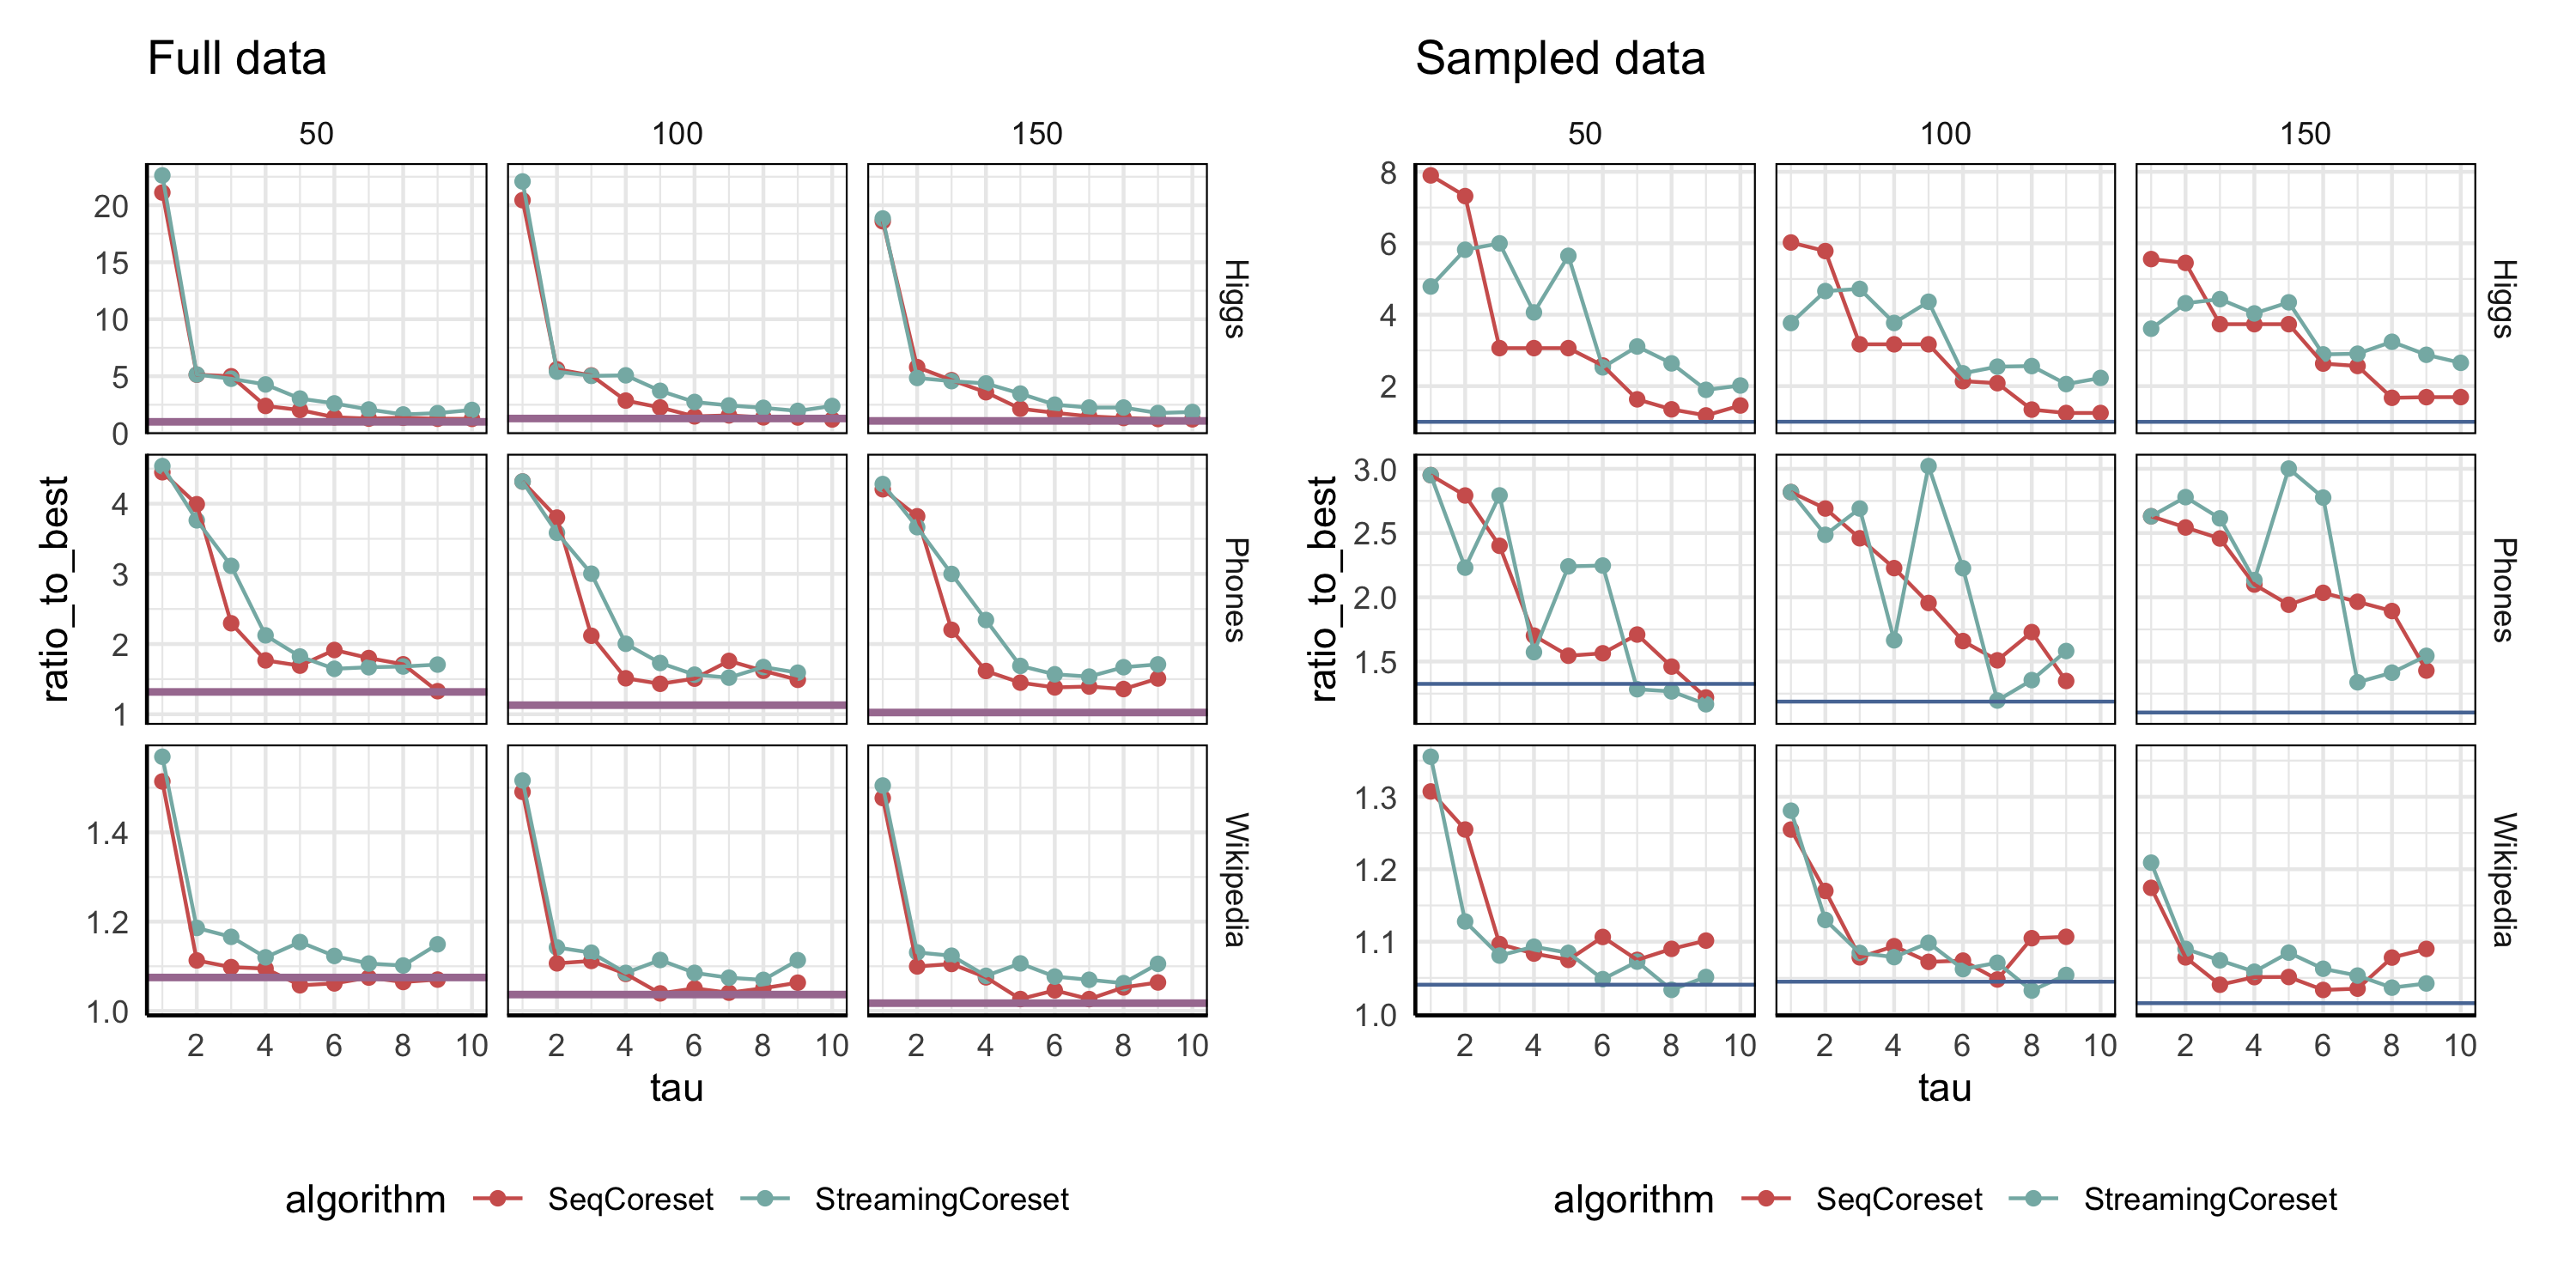
\includegraphics[width=\textwidth]{seq-effect}
    \caption{
        \label{fig:seq-effect}
        Effect of the parameter $\tau$ on the solution quality.
        There is an interplay between the matroid constraint and the allowed outliers, if we want to observe some effect of the parameter tau.
        In particular, we have that allowing for too many outliers (e.g. Wikipedia 0.0001, which is 500 outliers over 5 million points) makes all the solutions very similar, because the most extreme distances are just removed.
        If the matroid constraint is too stringent (i.e. there is too little liberty in choosing the centers)
        then the solutions will also be too similar to each other.
    }
\end{figure*}

First we consider the effect of varying the size of the coreset on the solution quality, in a sequential setting.
Due to the high complexity of \chen, we are unable to run it on the
full datasets, hence we also consider samples of 10\,000 points.
We vary $\tau$ from 1 to 10: note that $\tau=1$ is a degenerate configuration where the coreset is an arbitrary independent set.

Lacking exact solutions,
we evaluate the quality of the solution in terms of the ratio between the returned radius
and the smallest radius found on that dataset \emph{by any configuration}.

Figure~\ref{fig:seq-effect} reports the results of this experiment.
First, we observe that increasing $\tau$ quickly improves the solution before hitting a plateau, where
building larger coresets does not improve the quality of the solution.
On \higgs this effect is more pronounced, whereas for \wiki already using a small coreset yields a good-quality solution.
\mc{Check the following statement in the light of the new experiments.}
Furthermore, we notice that \stream and \seq have comparable quality, with the former performing slightly 
worse for the same coreset size, as predicted by the theory.

Comparing with \chen (blue horizontal line) on the sampled datasets, both \seq and \stream compute comparable, 
if not better, solutions using rather small coresets.
As we shall see,
using small coresets has a dramatic effect on the running time.

\begin{figure*}
    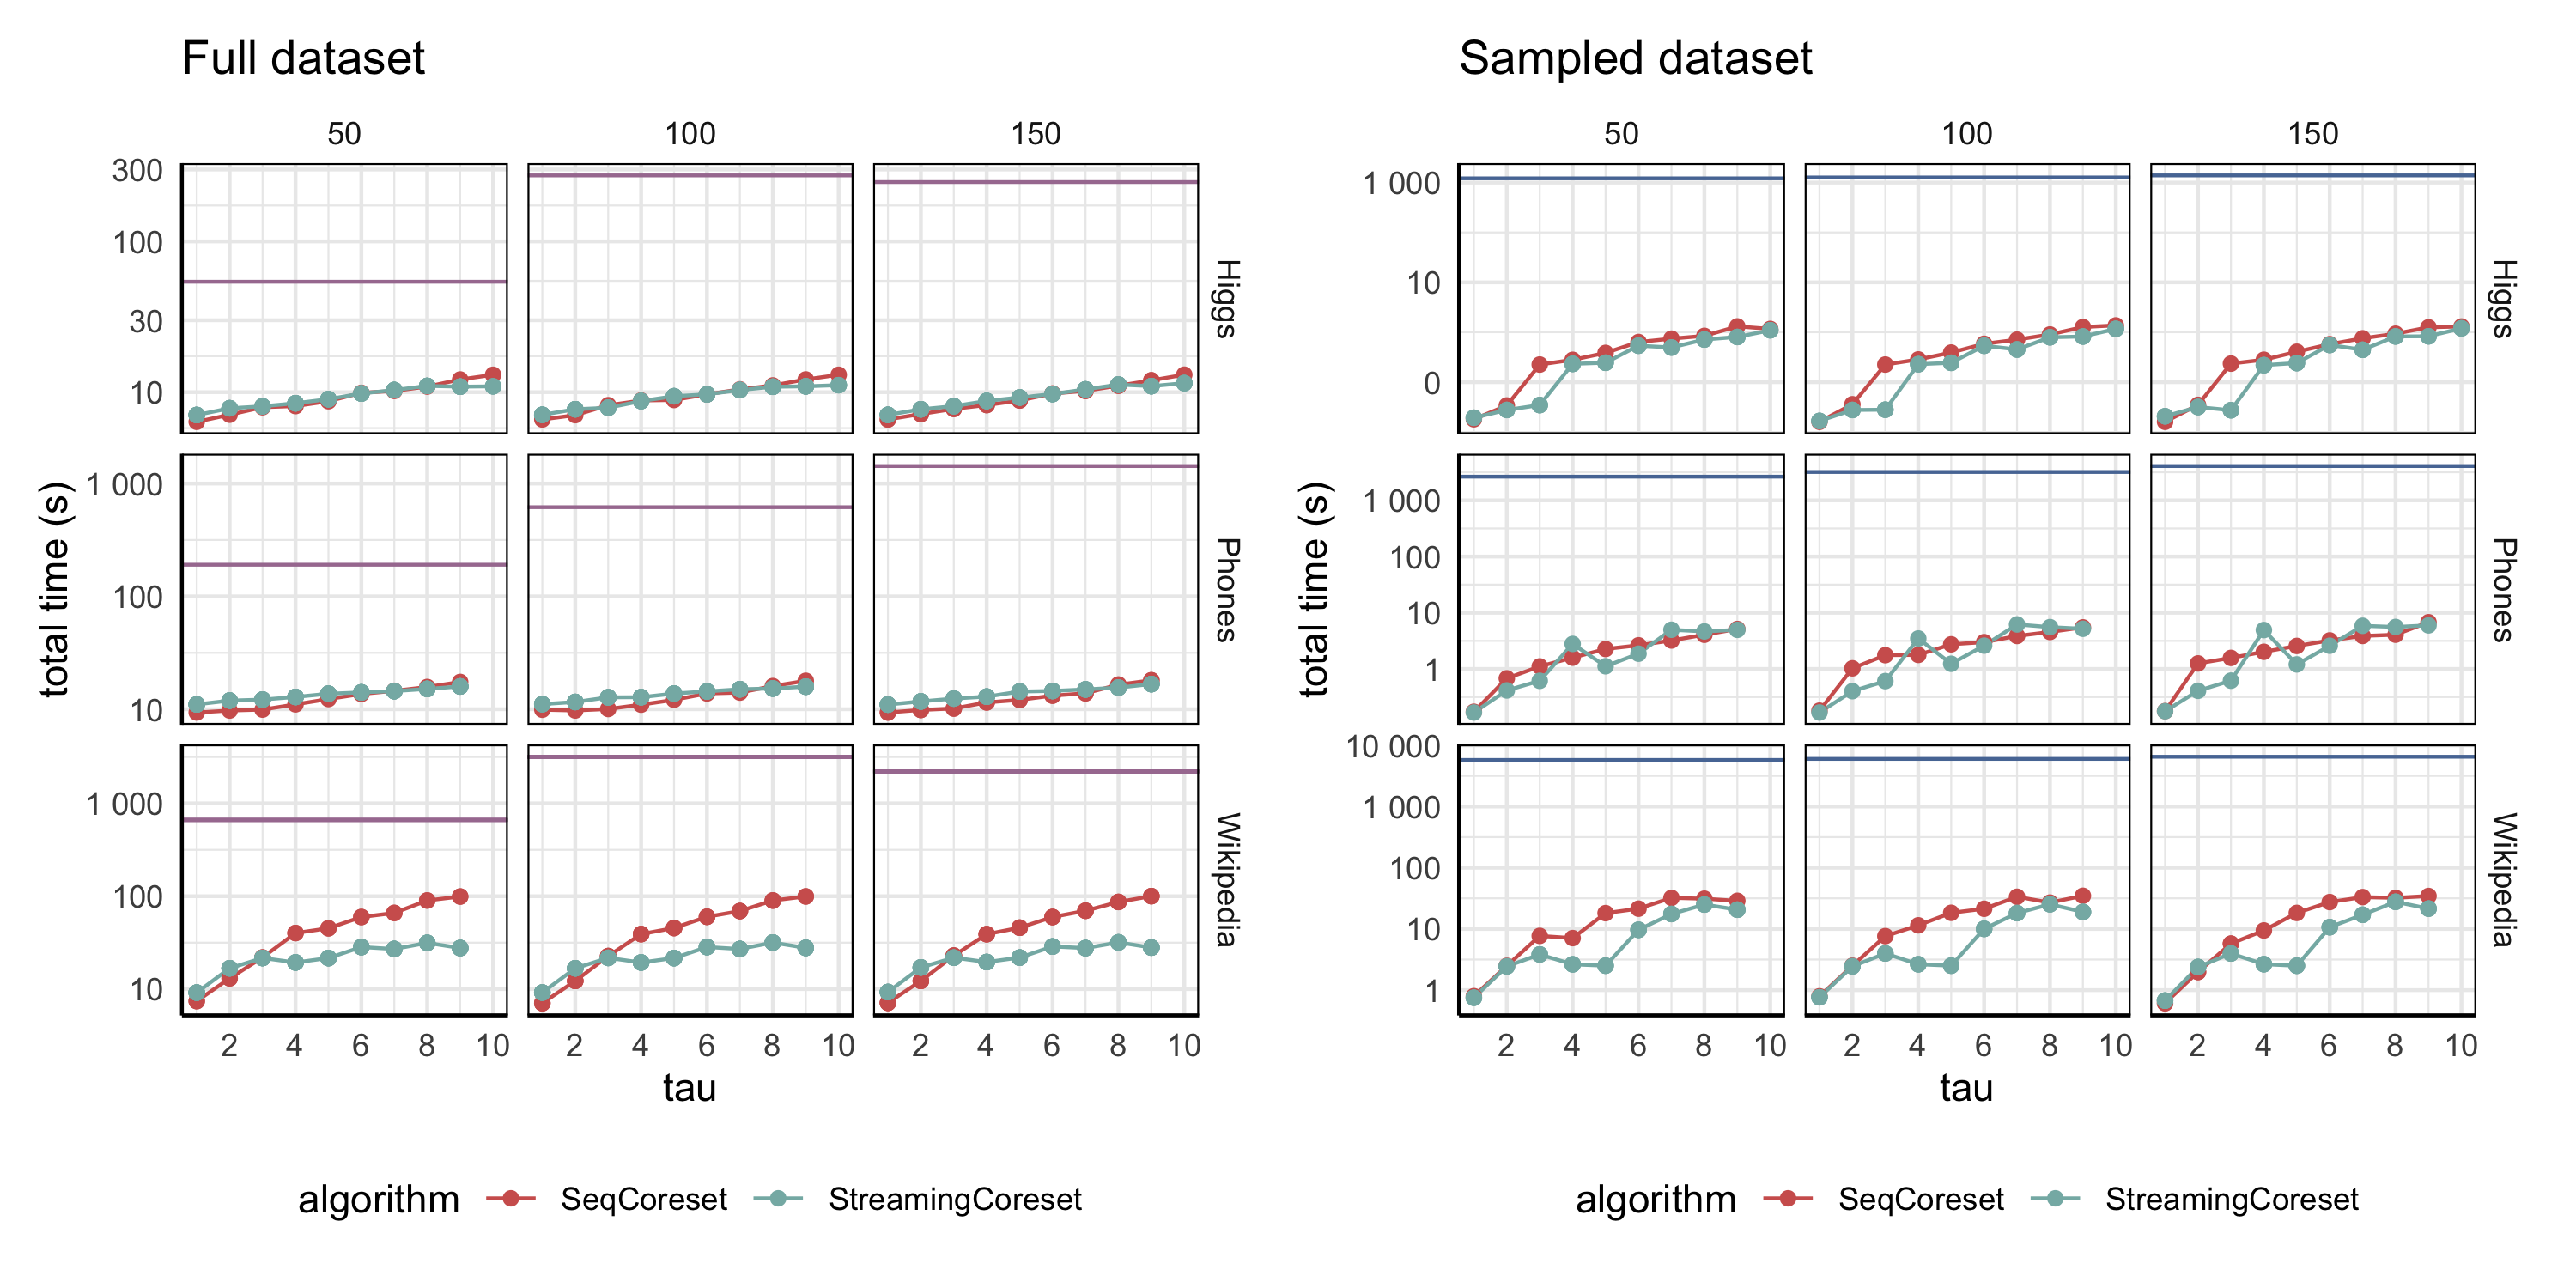
\includegraphics[width=\textwidth]{seq-time}
    \caption{
        \label{fig:seq-time}
        Effect of the parameter $\tau$ on the total running time.
    }
\end{figure*}
Figure~\ref{fig:seq-time} reports the running times of these experiments,
showing that coreset based approaches are between two to three orders of magnitude faster than \chen
(on samples of 10\,000 points of each dataset) for values of $\tau$ giving solutions of comparable quality.
As for the relative performance of \seq and \stream, on sampled datasets they have similar performance.
\mc{Reformulate this in the light of the new experiments.}
On the full datasets, \seq has a very predictable performance, degrading for increasing values of $\tau$.
The performance of \stream, on the other hand, is almost constant in $\tau$, and slower than $\seq$.
We emphasize, though, that \stream can work with unbounded inputs.

\subsection{Memory requirements}
\label{sec:memory}

\begin{figure}
    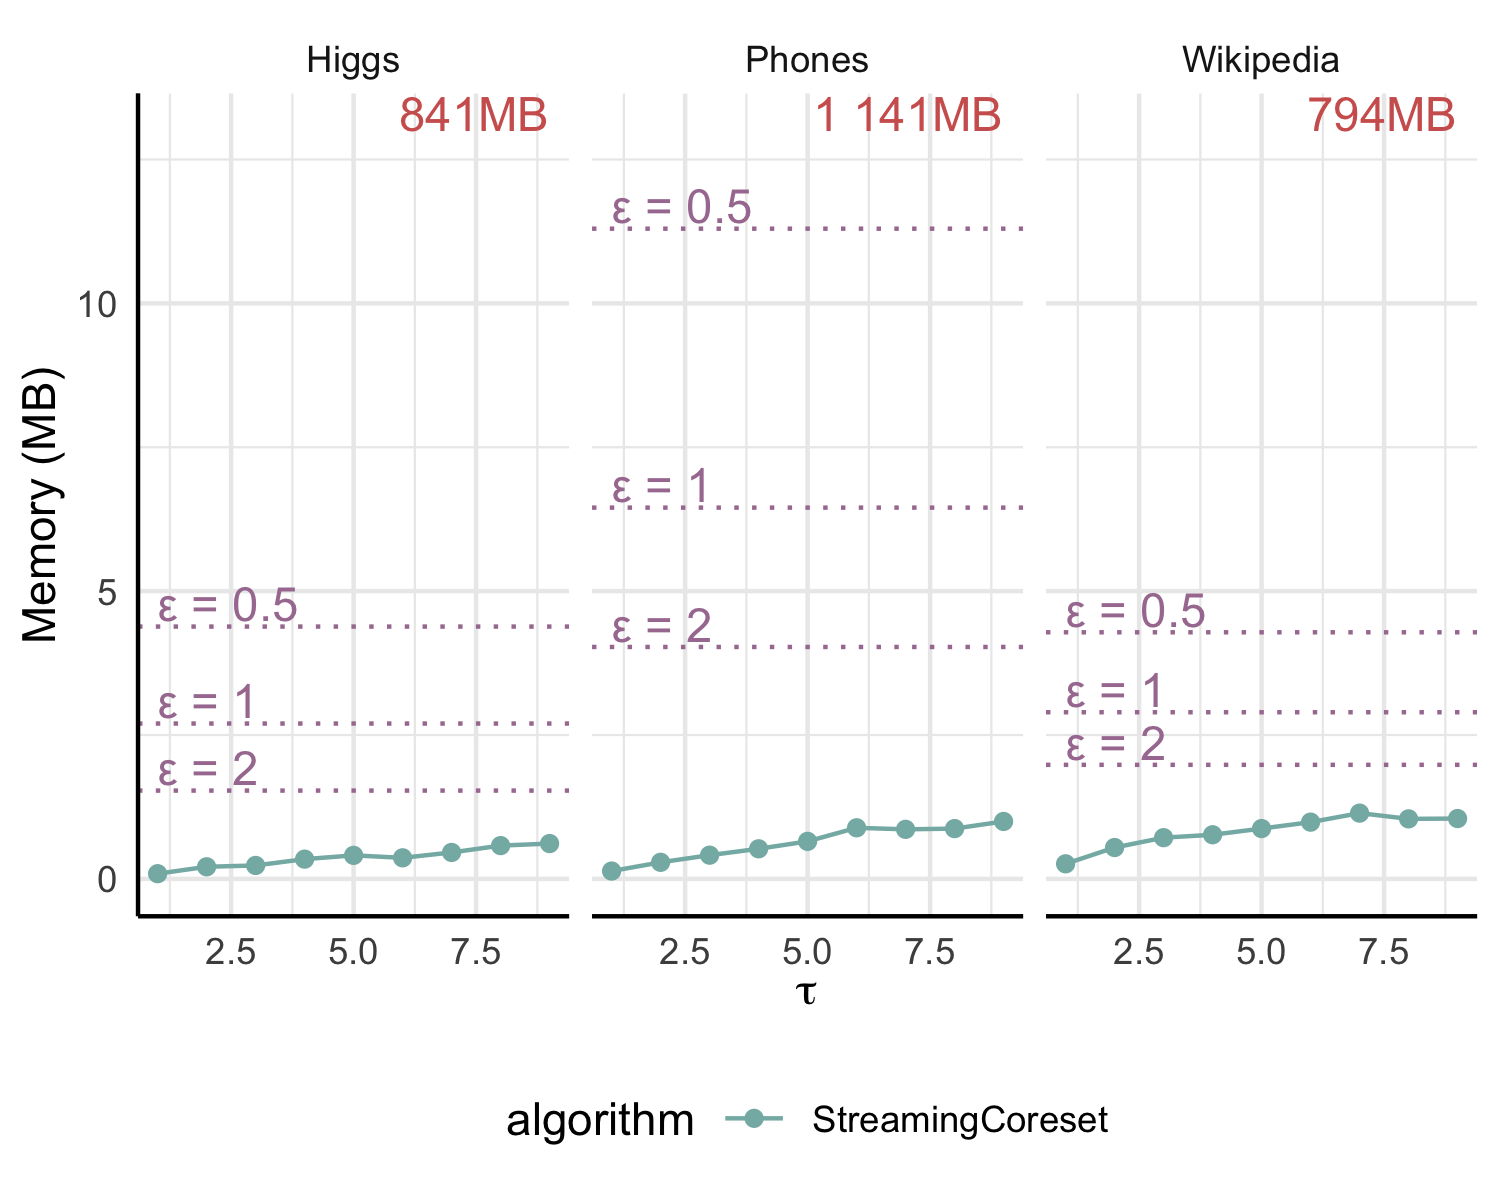
\includegraphics[width=\columnwidth]{memory}
    \caption{\label{fig:memory}Memory required by \stream and \seq to build the coreset.}
\end{figure}

In this section we focus on the memory required by \seq and \stream to build the
coreset.
In particular, recall that \seq needs to store the entire dataset in memory, whereas \stream 
can work with a small working memory.
Figure~\ref{fig:memory} reports on the results of this experiments, for varying values of $\tau$
and fixing the number of outliers to 150 (which does not influence the coreset construction memory).


\subsection{Scalability of the MapReduce coreset construction}
\label{sec:exp:mapreduce}

\begin{figure*}
    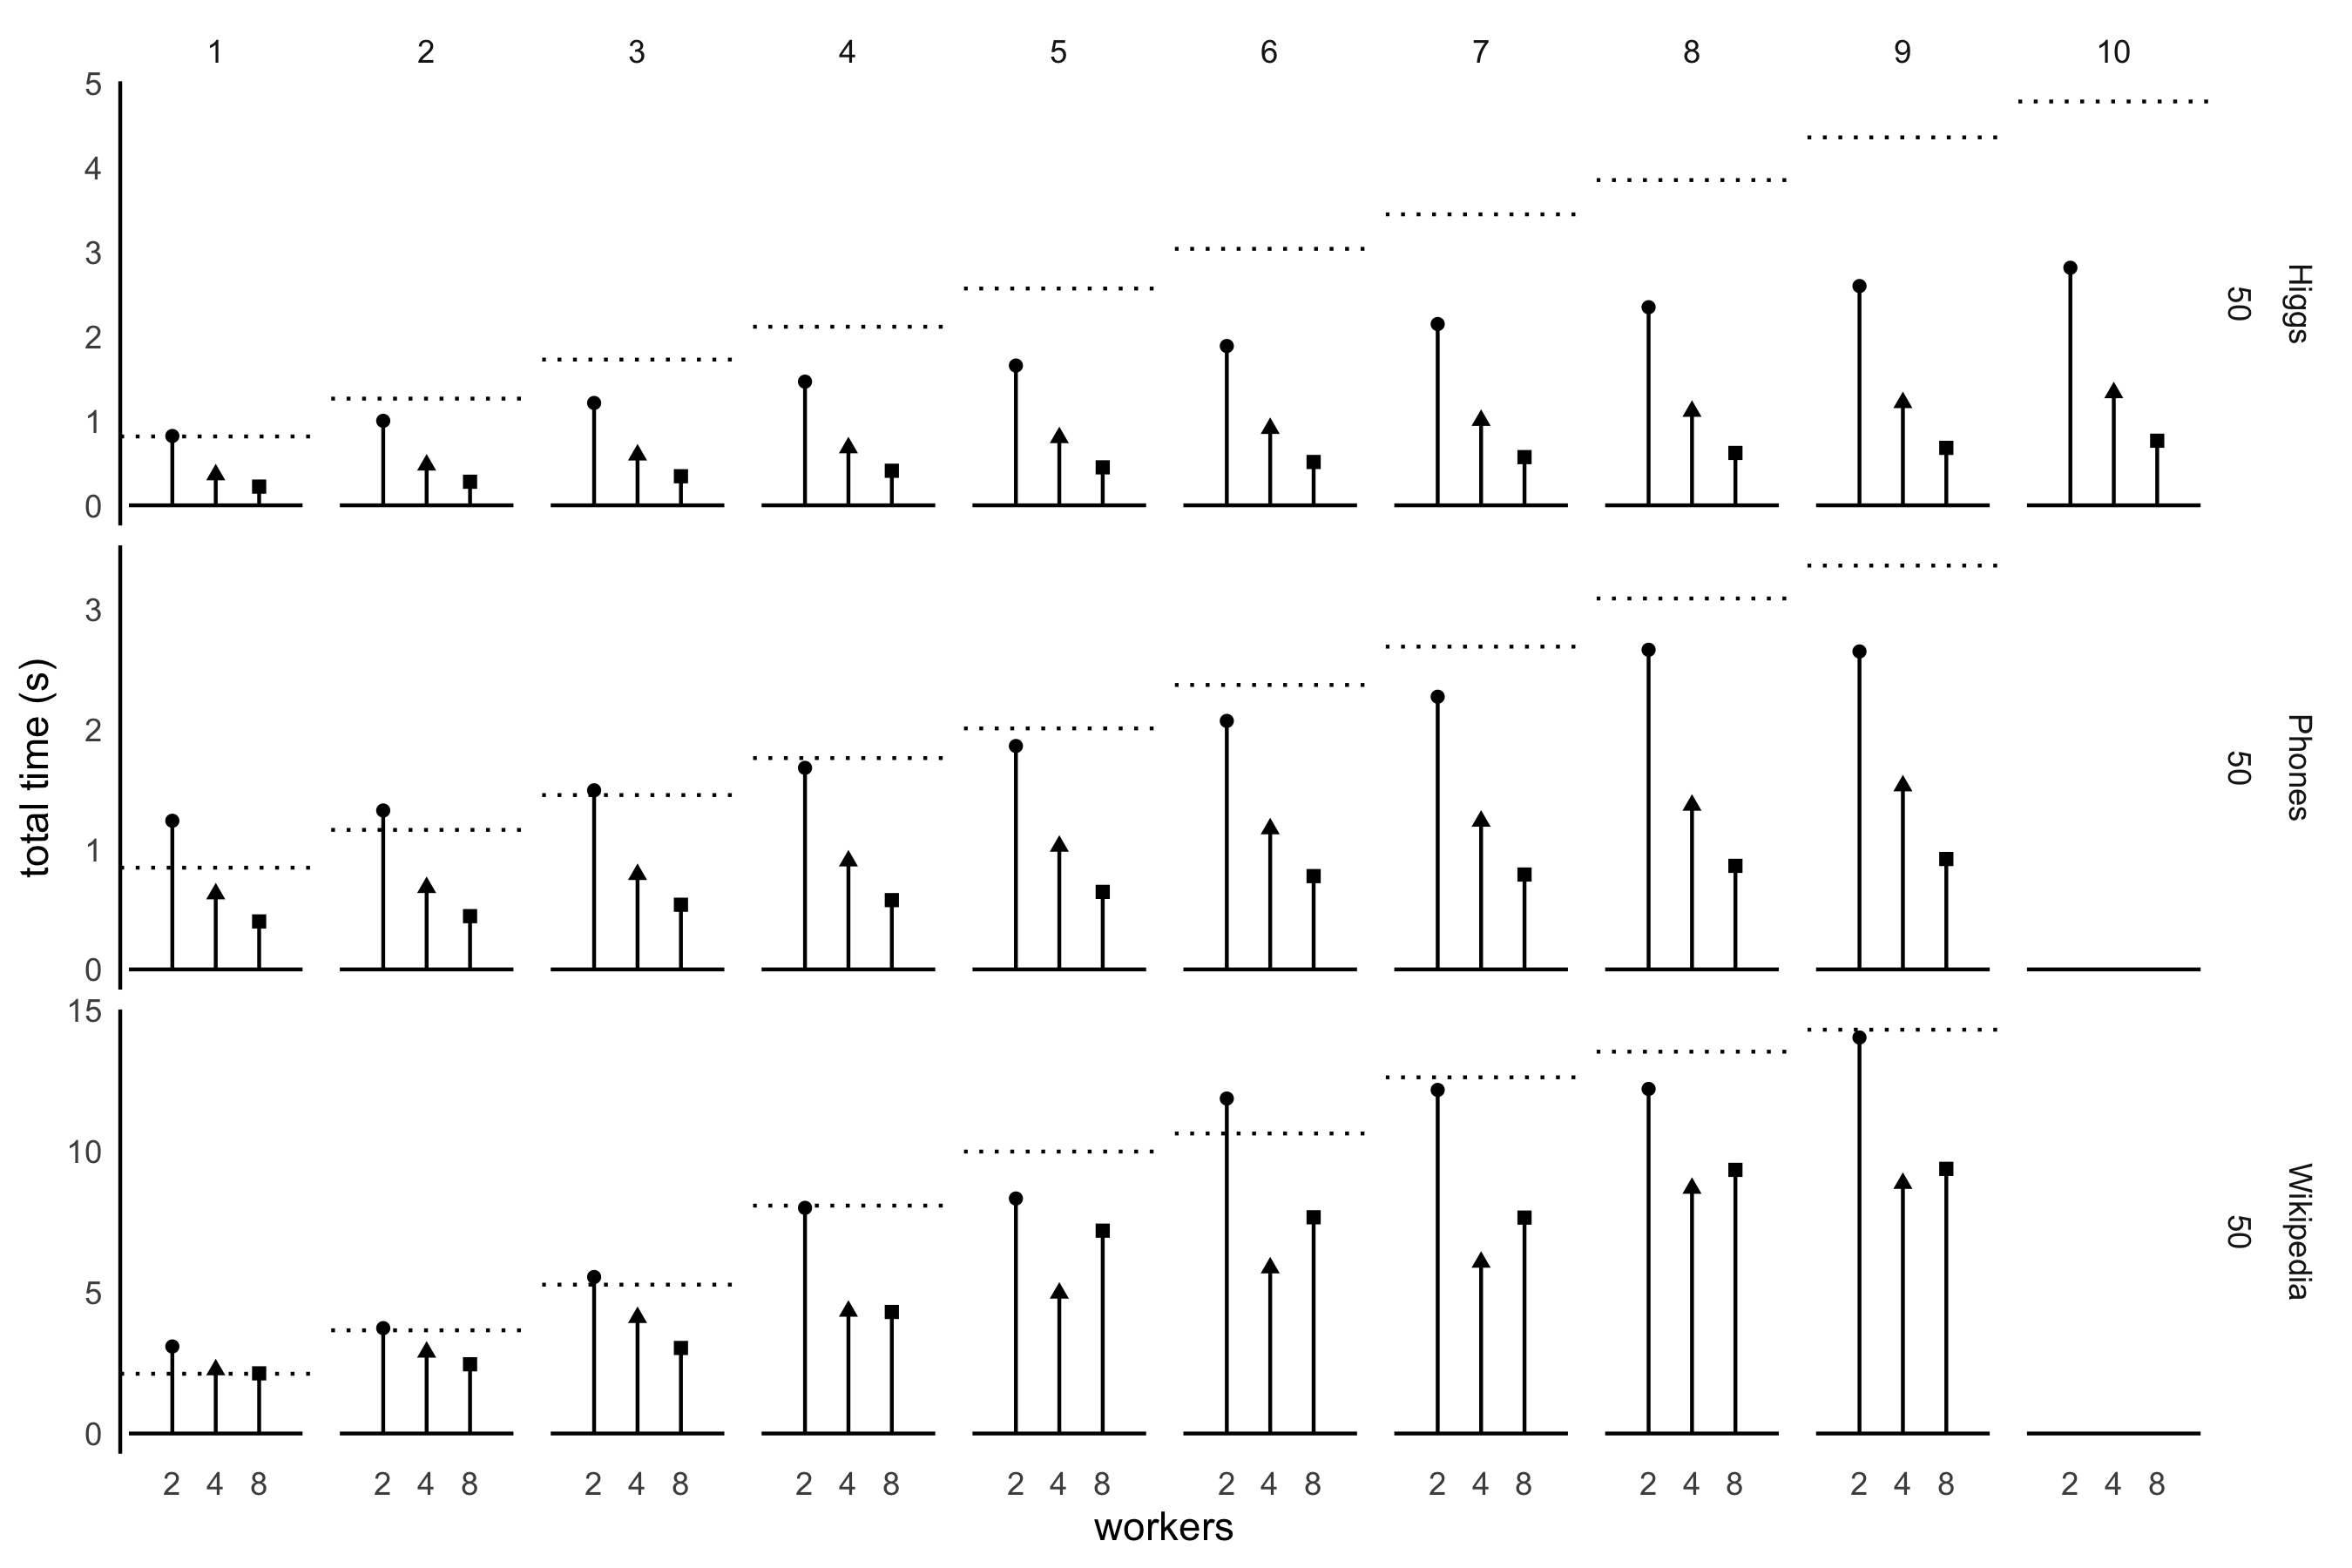
\includegraphics[width=\textwidth]{mr-time}
    \caption{
        \label{fig:mr-coreset-time}
        Time to build the coreset with the \mapr algorithm, for varying number of workers.
        Each column of plots corresponds to a different value of $\tau$.
        The dotted line represents the performance of the \seq algorithm in constructing the coreset.
        The time scale is linear.
        \mc{Computing the solution on the coreset is one order of magnitude slower than
        building the coreset itself, hence we don't report that time here in this figure.}
        The construction of the coreset scales linearly for Higgs and Phones: doubling 
        the resources halves the running time, also starting from the sequential baseline 
        (dotted line). For Wikipedia the scalability is 
        less pronounced, due to the higher cost of invoking the matroid oracle.
        \mc{Show fewer values of $\tau$ in the final version.}
    }
\end{figure*}

We now focus on the cost of building the coreset using the \mapr algorithm, compared to \seq.
We test 2, 4, and 8 workers, varying the values of $\tau$ between 1 and 10. Note that for the same value
of $\tau$, the size of the aggregated coreset will change depending on the number of workers.
As for the number of allowed outliers, we fix it to 50, noting that it does not influence the 
time required to build the coreset itself.

Figure~\ref{fig:mr-coreset-time} reports the results of this experiment. 
For a fixed value of $\tau \ge 3$, on \higgs and \phones the \mapr construction scales linearly with the 
number of processors. 
The \seq algorithm is faster than \mapr with 2 workers for small values of $\tau$. 
This is due to the overheads introduced by the communication required to distributed data to
processors located on different machines.

The scalability is less pronounced for \wiki, mainly due to the higher cost of evaluating the matroid oracle.
\mc{In fact, for larger values of $\tau$, the algorithm scales only from 2 to 4 workers, 
    and slows down when going from 4 to 8 workers. This is a behavior to be investigated}

\subsection{Time to compute the solution}

\begin{figure}
    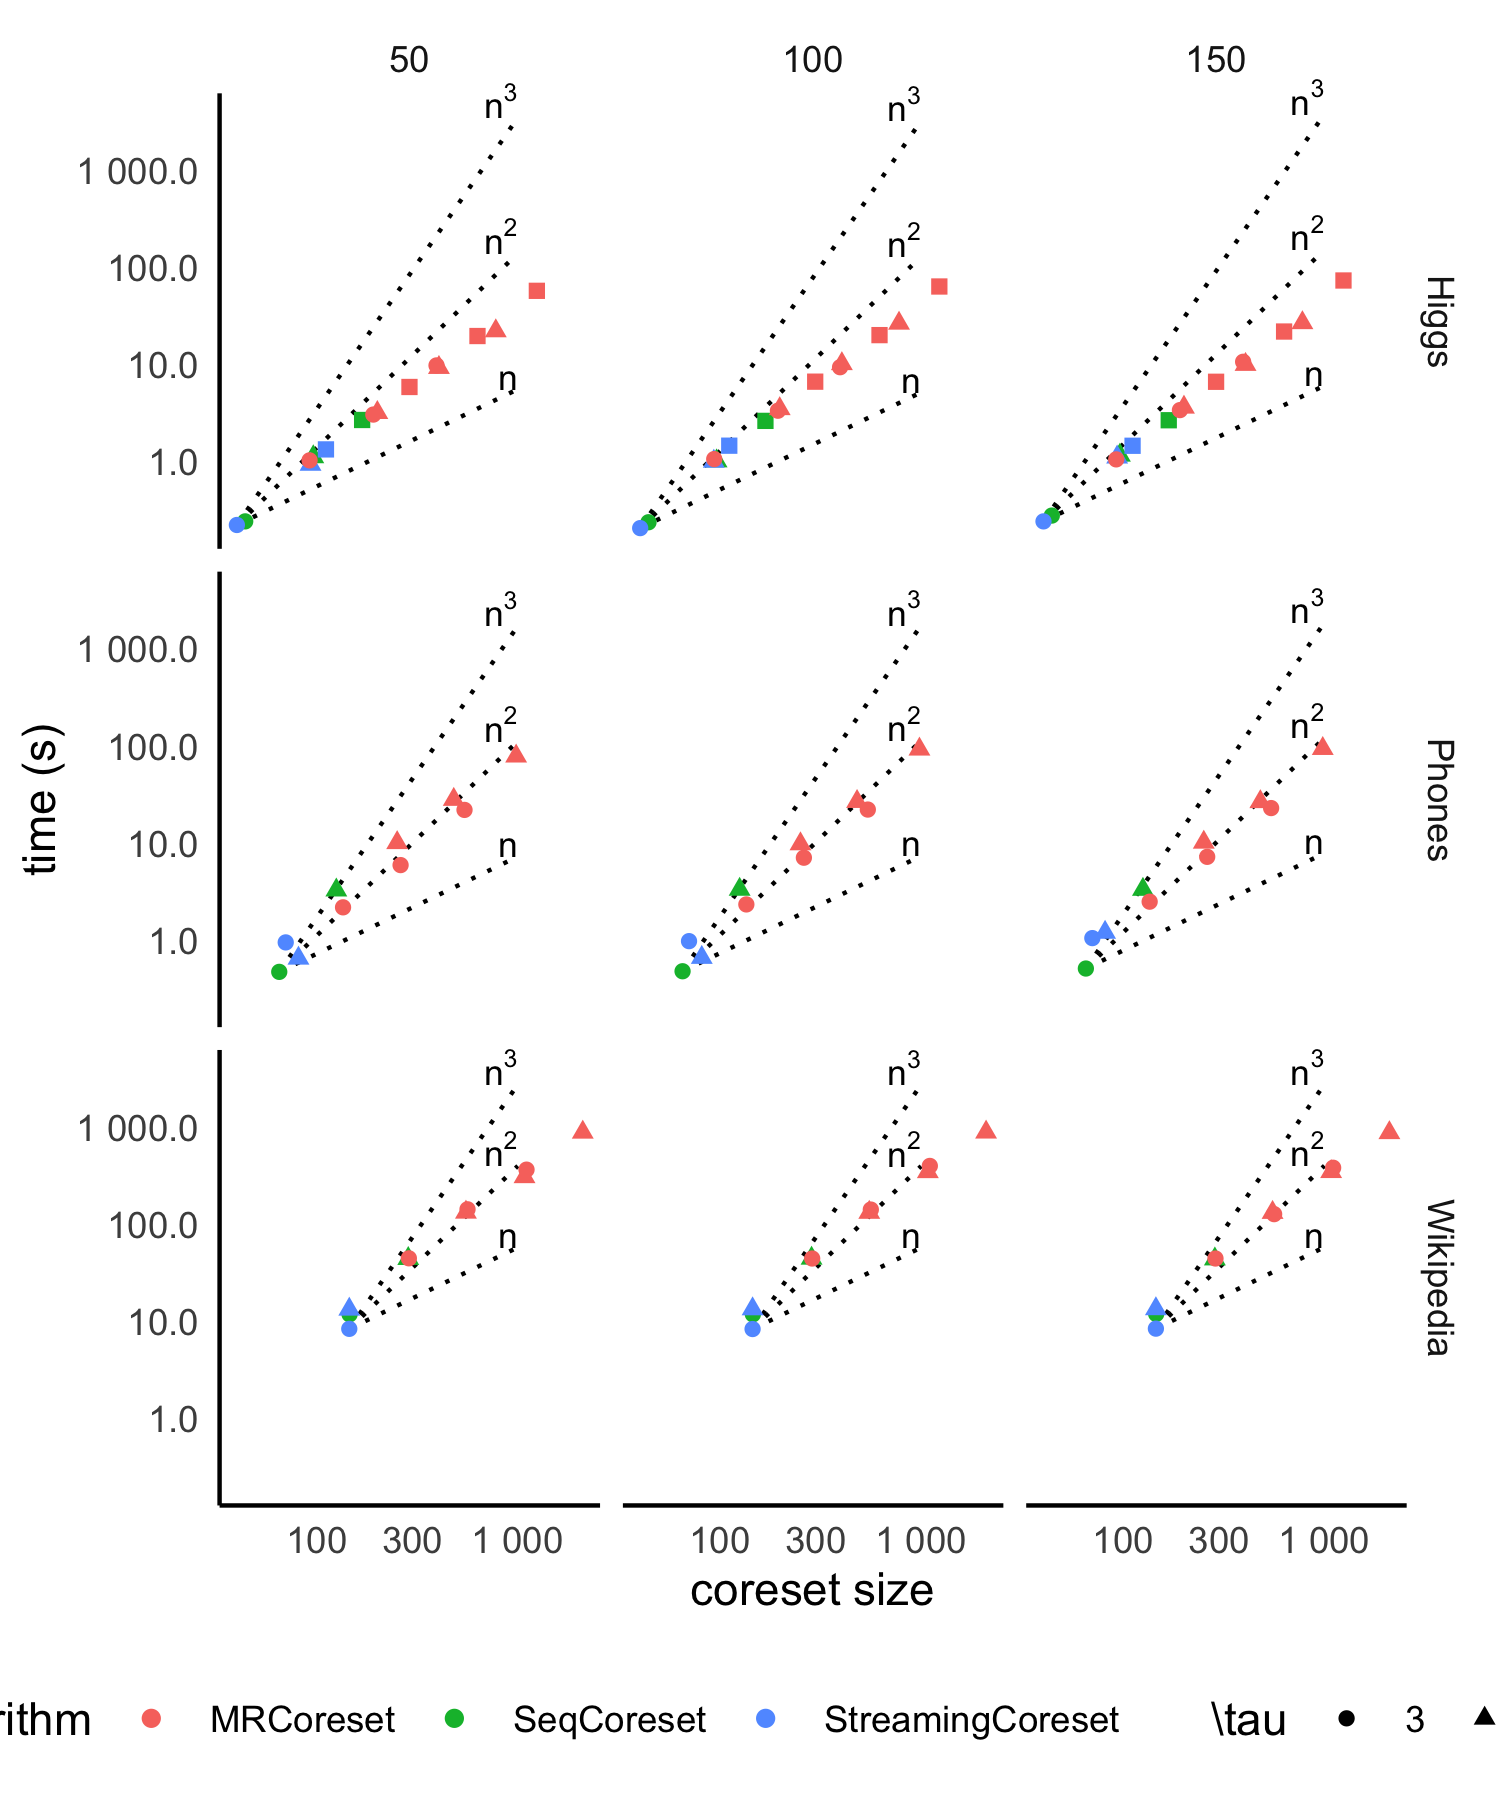
\includegraphics[width=\columnwidth]{solution-time.png}
    \caption{
        \label{fig:solution-time}
        Time to compute the solution on the coreset against coreset size.
        The scale is logarithmic on both axes.
    }
\end{figure}

Finally, we consider the time to compute the clustering solution on the coreset, and 
how it compares with computing the coreset in the first place.
Figure~\ref{fig:solution-time} reports the time required to compute the clustering
solution against the size of the coreset.

\begin{figure}
    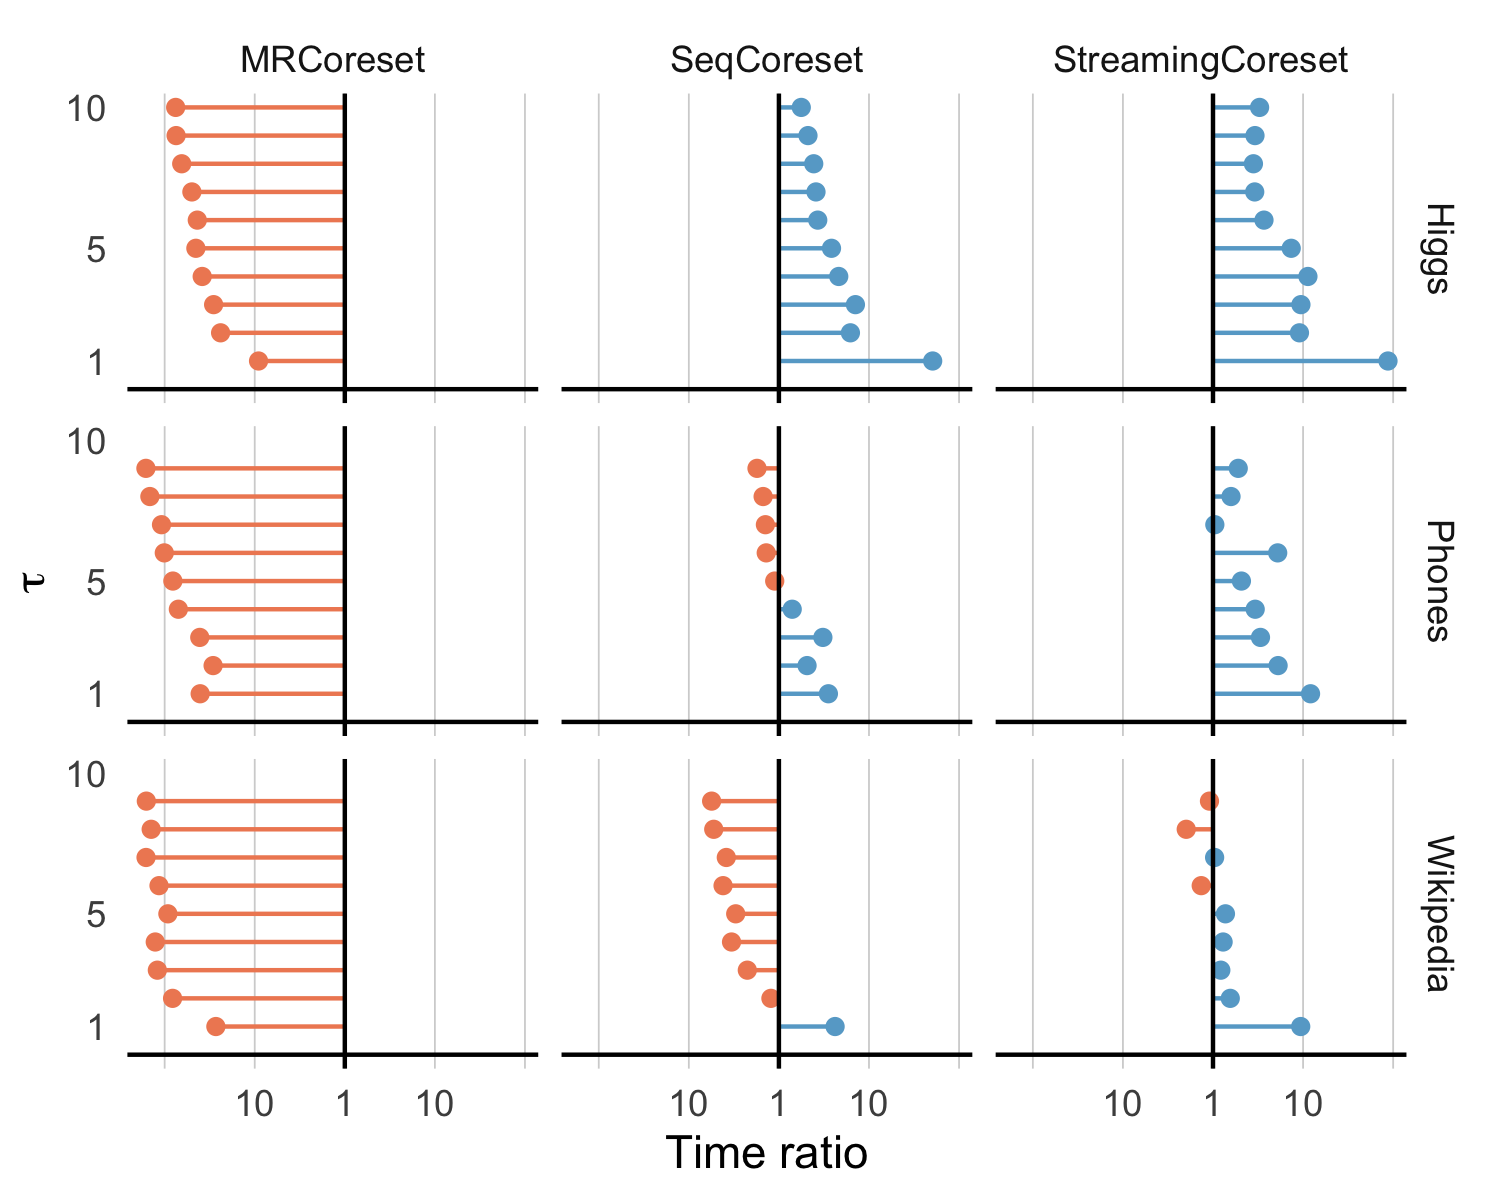
\includegraphics[width=\columnwidth]{time-ratio.png}
    \caption{
        \label{fig:time-ratio}
        Ratio between the time spent building the coreset and time spent computing the solution.
        To the left the time for the solution dominates, to the right the time spent for the
        coreset dominates.
    }
\end{figure}
We now observe the ratio between the time required to compute the coreset and the time to compute the 
solution.
In \mapr we fix the number of workers to 8.
The results are reported in Figure~\ref{fig:time-ratio}, where each line corresponds to a value of $\tau$
for a given combination of algorithm and dataset.
Lines leaning toward the left represent configurations where the computation of the solution is more expensive,
lines directed toward the right are configurations where the running time is dominated by the coreset construction.
Note that for a fixed value of $\tau$ the coreset computed by \mapr are a factor 8 larger, since that is the number
of machines employed in parallel.

In general, we note that building larger coresets tilts the balance between more expensive 
computation of the solutions. This is expected: the coreset construction scales linearly in $\tau$,
whereas the computation of the solution suffers from a quadratic complexity, as we have 
seen in Figure~\ref{fig:solution-time}.
In particular, the larger coresets built by \mapr require very little time to build in practice,
but imply a larger (in proportion) solution time.
